\chapter{Additional Results}\label{app:additional_results}


\section{Models Learn Most Significant Digits First}
Interestingly, over the duration of training, first model gets the digit in most significant position right, and then gets more and more digits right towards the least significant. This is also seen in loss, which drops in steps. This is not because in sampling, the most significant digit is output first (left-to-right), since the effect also happens (in reverse) when the answer is reversed!

\begin{figure}[ht]
    \centering
    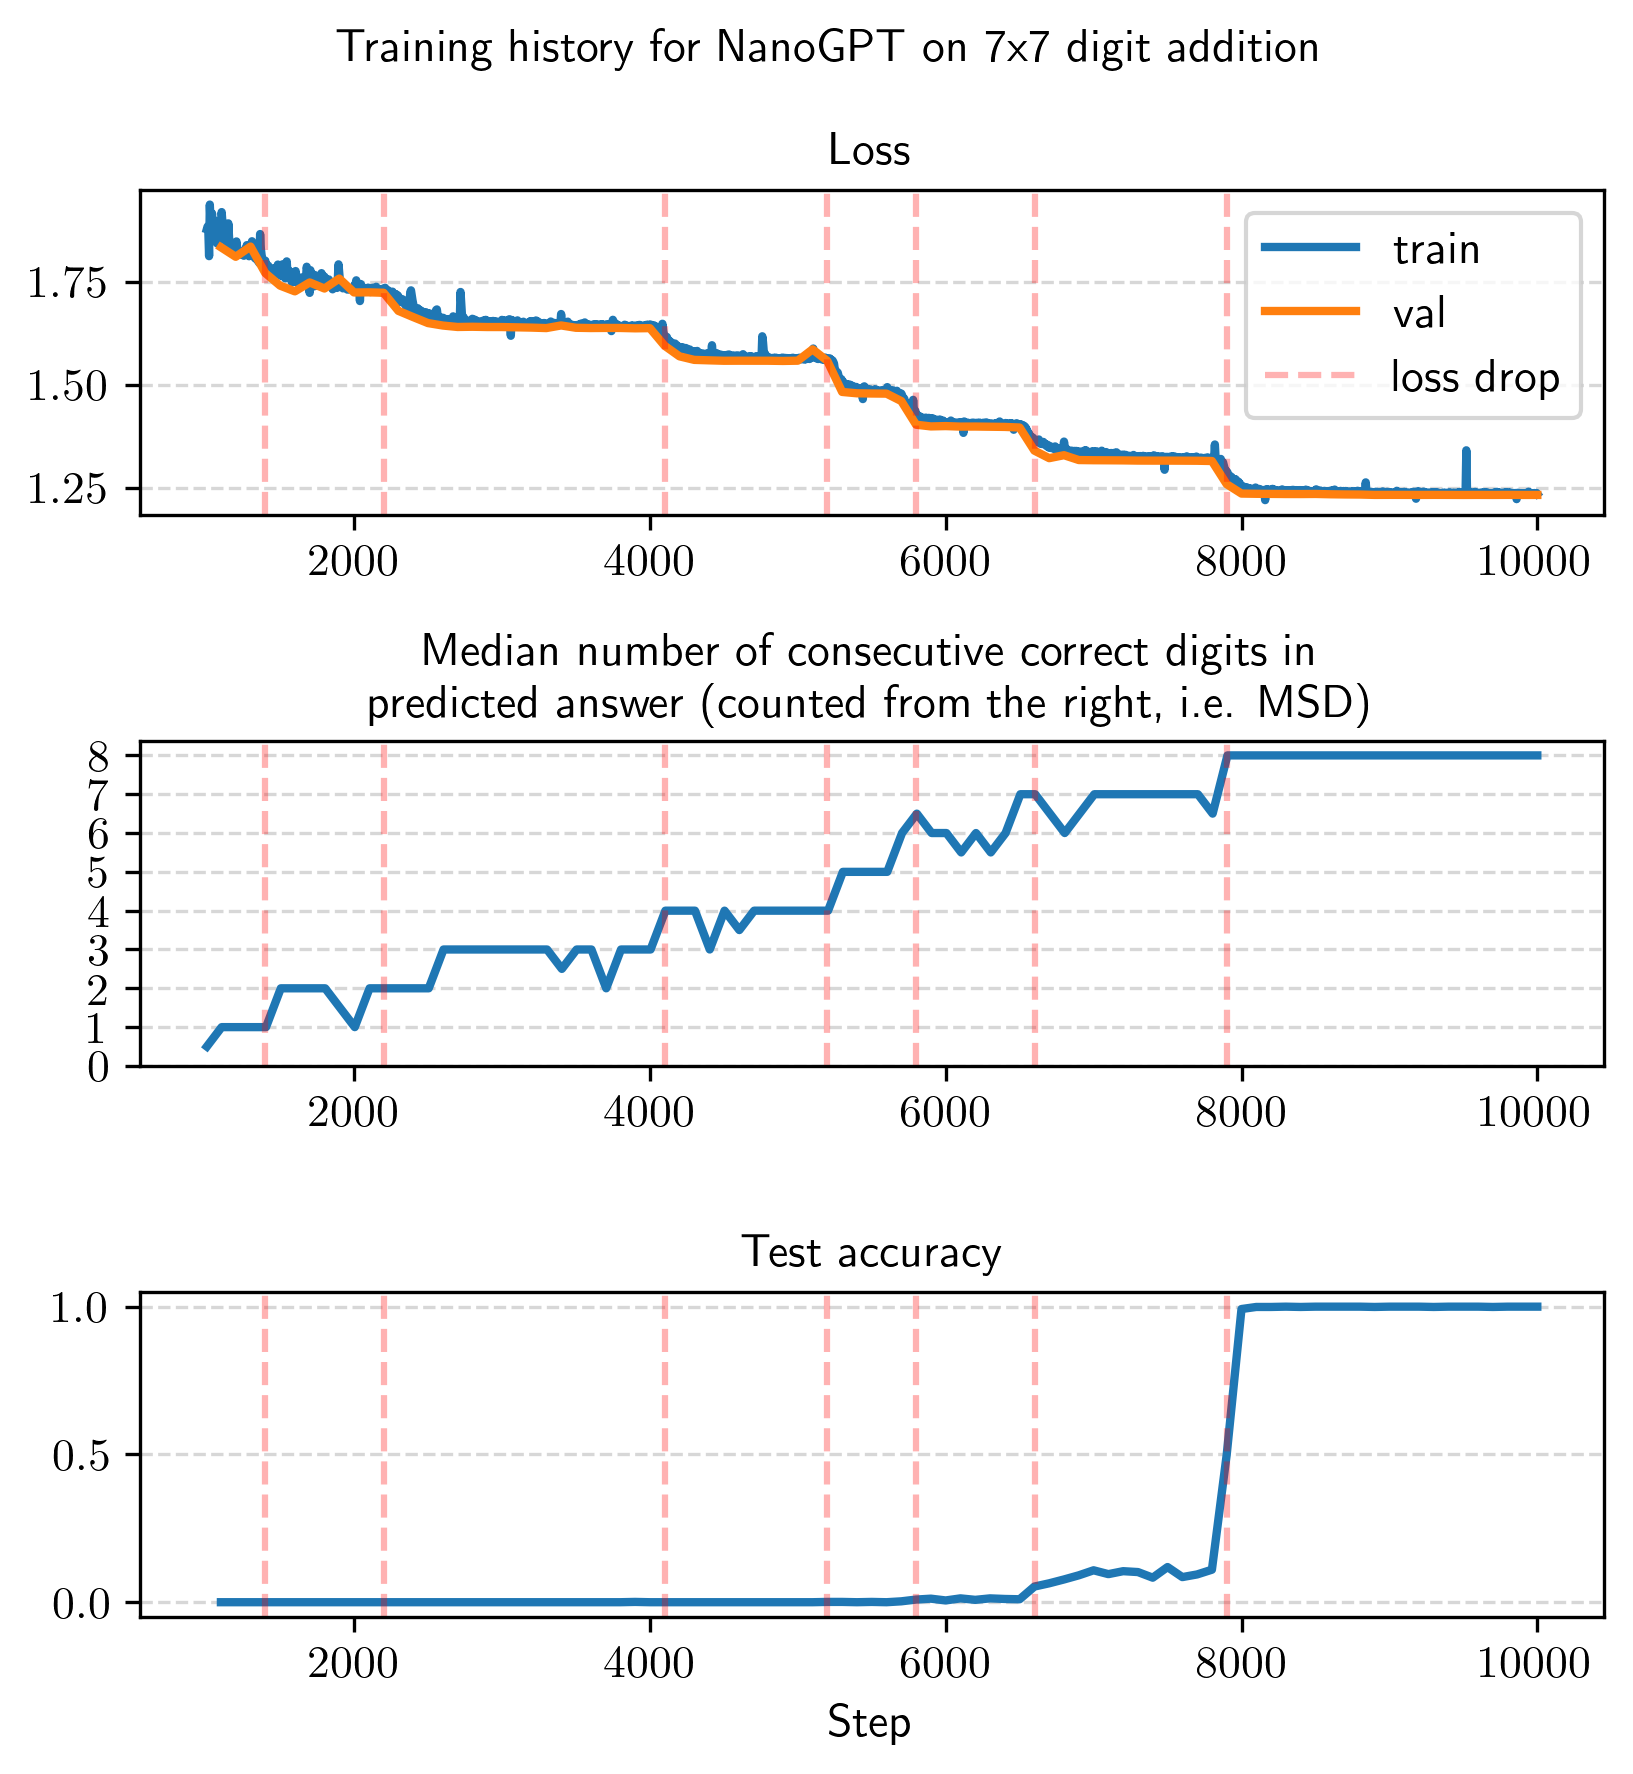
\includegraphics[width=0.8\textwidth]{fig/digitwise_loss.png}
    \caption{Loss drops in NanoGPT decoder-only model with absolute position encoding training that correspond to the model learning the digit positions one by one from most significant to least significant. Accuracy is boosted after model learns all of the digit positions.}
    \label{fig:digitwise_loss}
\end{figure}
